\begin{frame}{Реализация упрощённой системы}
    \begin{itemize}
        \item Нужна для понимания, как работает Nanite
        \item Преобразование меша в граф --- долгий предподсчёт
        \item Разбиение меша с помощью библиотеки METIS
        \item Невозможно задать жёсткое ограничение на размер мешлета, поэтому количество мешлетов берётся с запасом
        \item Отрисовка --- Mesh Shader в DirectX 12
    \end{itemize}
\end{frame}

\begin{frame}{Реализация: скриншоты}
    \begin{center}
        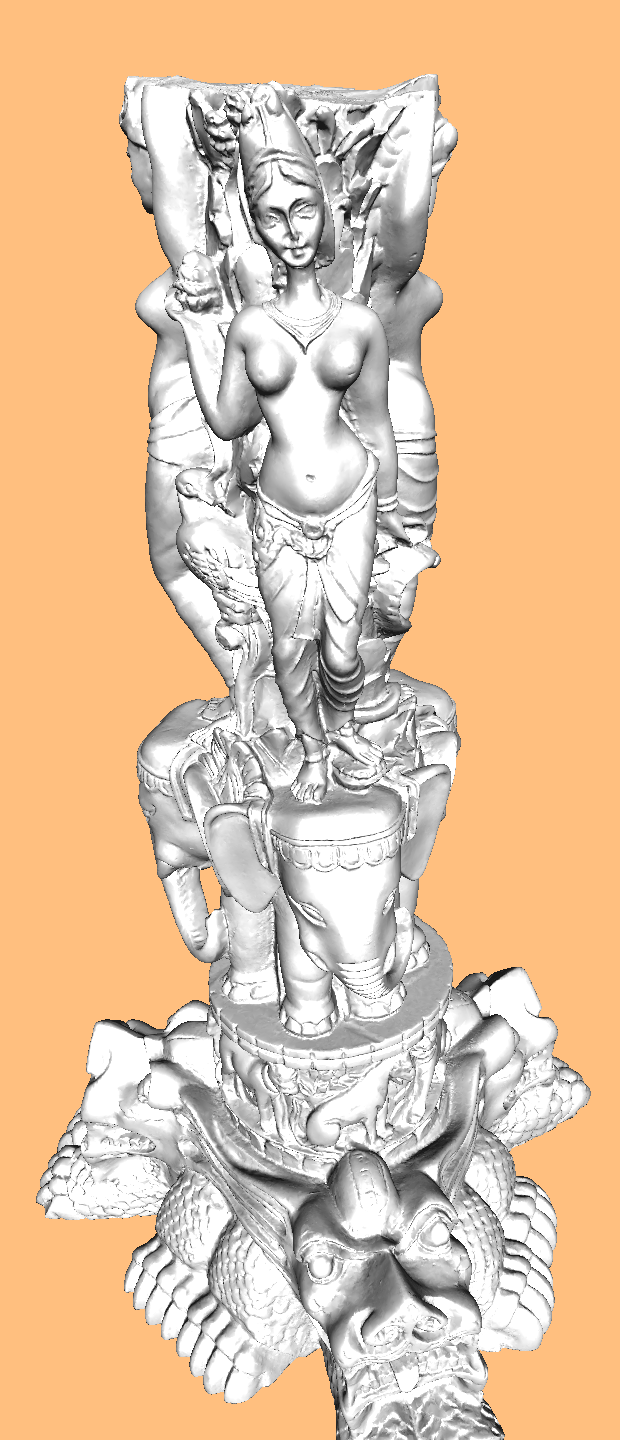
\includegraphics[width=.2\textwidth]{demo-cut-0.png}
        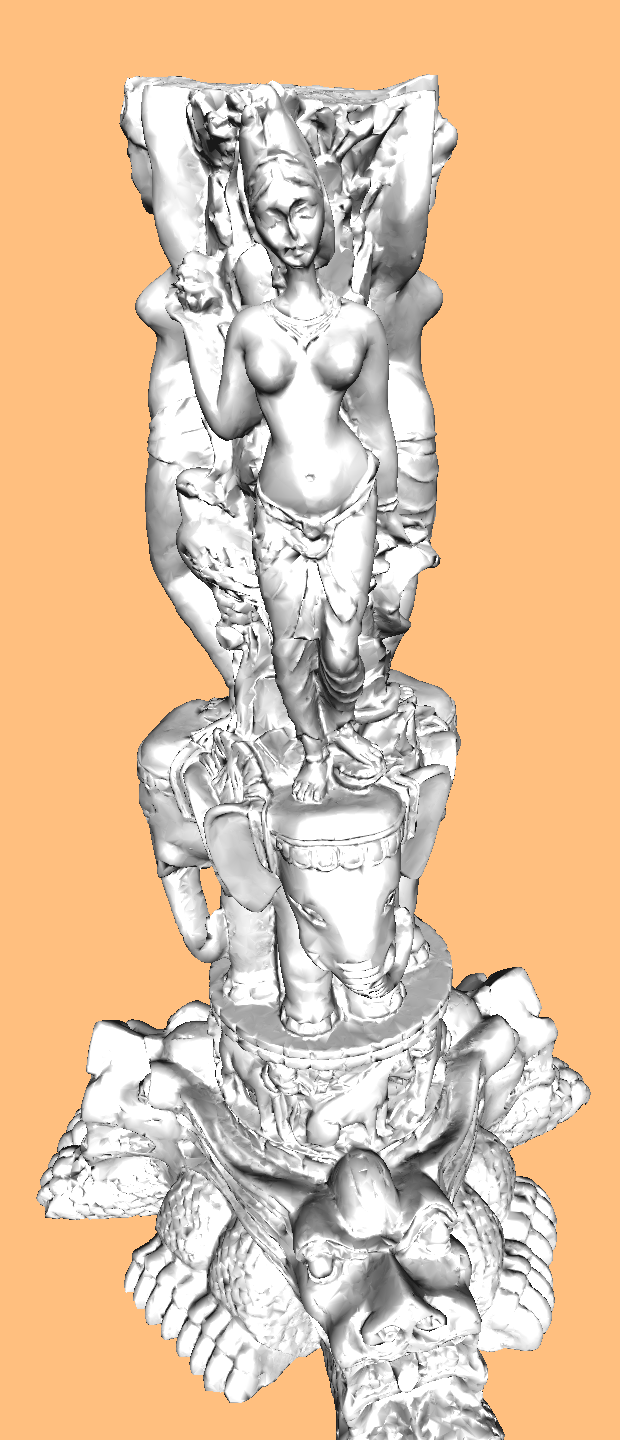
\includegraphics[width=.2\textwidth]{demo-cut-1.png}
        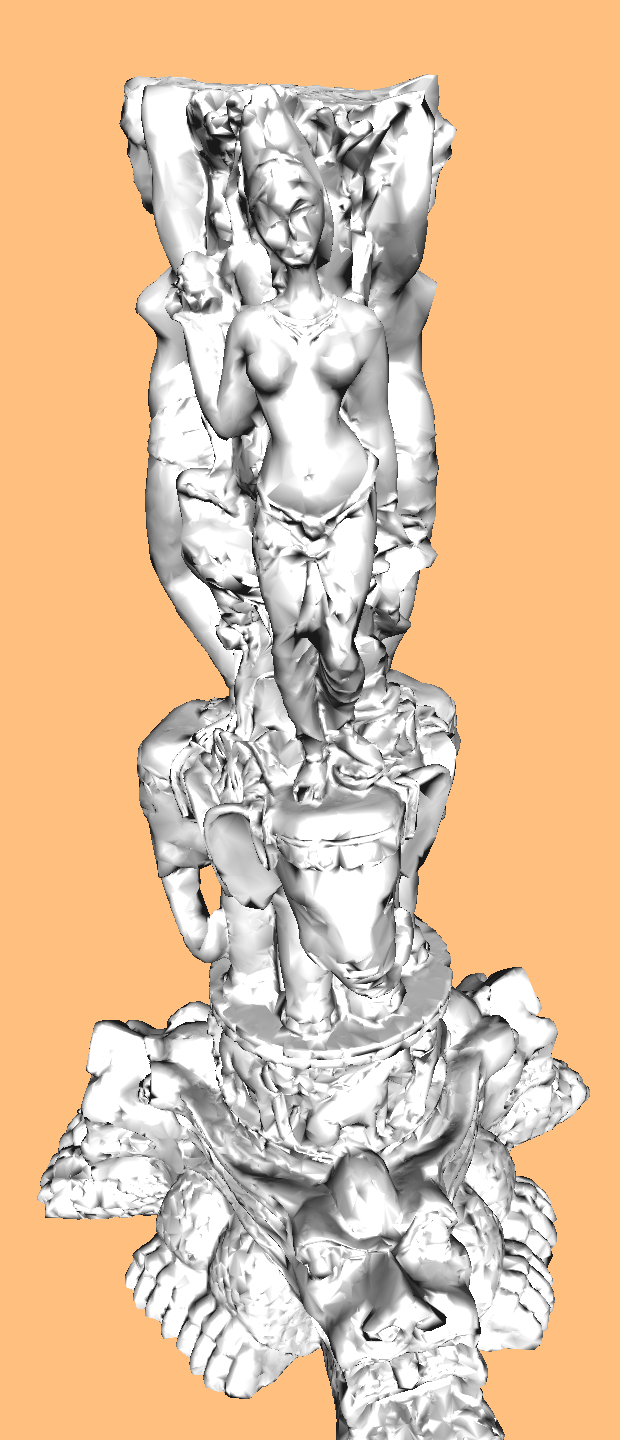
\includegraphics[width=.2\textwidth]{demo-cut-2.png}
        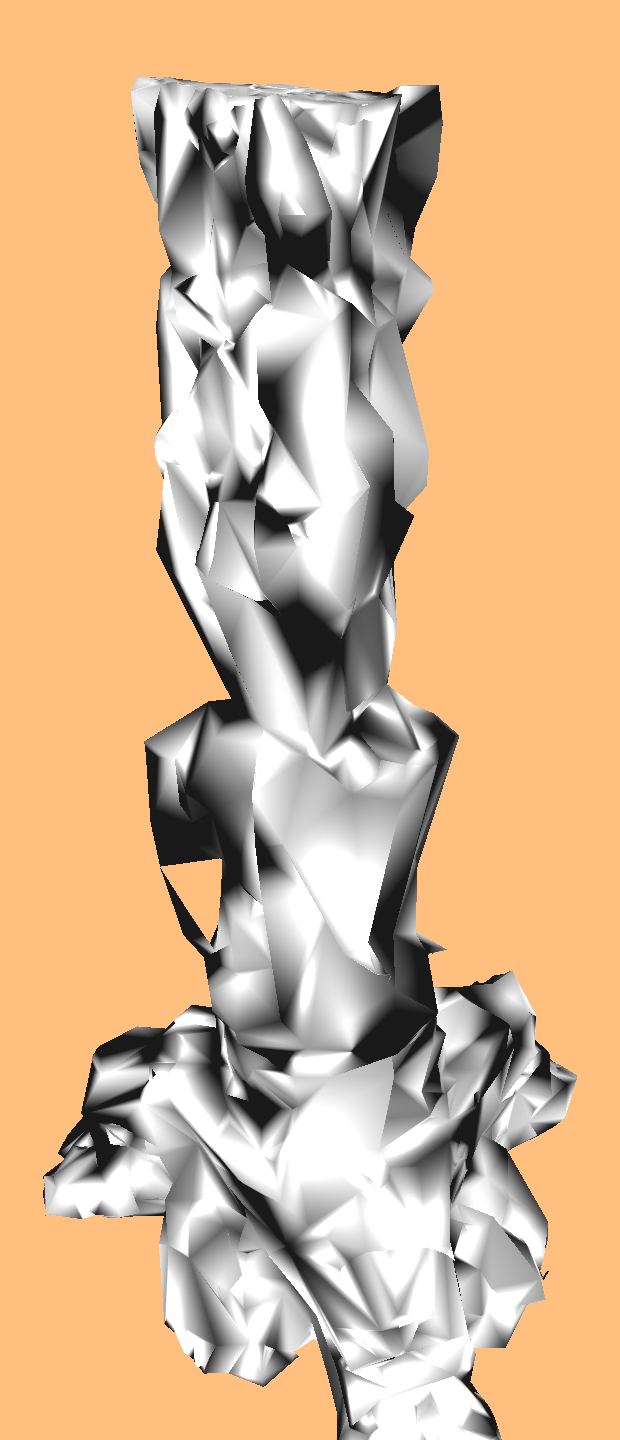
\includegraphics[width=.2\textwidth]{demo-cut-3.png}
    \end{center}
\end{frame}
